\chapter{Diseño e implementación del sistema de \textit{scripts}}
\label{cap:diseñoImplentacion_scripts}

% Corregido 29/12/2023
% Revisado 14/01/2024

Como he explicado en el capítulo \ref{cap:introducion}, el objetivo principal de este
proyecto es poder generar código en C a partir de un fichero ejecutable. Para poder
alcanzar este objetivo nos asistiremos con inteligencia artificial de tal manera que
podamos conseguir resultados óptimos. Para ello, deberemos de generar un \textit{dataset}
que contenga los datos necesarios para poder entrenar nuestro modelo.

Se ha diseñado un sistema de \textit{scripts} que nos permitirá automatizar el proceso
de generar nuestro \textit{dataset}. Para el diseño de este sistema se han seguido los
siguientes criterios:

\begin{itemize}
    \item \textbf{Modularidad:} el sistema de \textit{scripts} debe de ser modular, de tal manera
        que se puedan añadir nuevas funcionalidades de manera sencilla.
    \item \textbf{Mantenibilidad:} el sistema de \textit{scripts} debe de ser mantenible, de tal
        manera que se puedan corregir errores o añadir nuevas funcionalidades de manera
        sencilla.
    \item \textbf{Portable:} el sistema de \textit{scripts} debe de ser portable, de tal manera
        que se pueda ejecutar en cualquier sistema operativo.
\end{itemize}

\section{Diseño del sistema de \textit{scripts}}
\label{sec:diseño_sistema_scripts}

% Corregido 30/12/2023
% Revisado 14/01/2024

Como bien he mencionado en el apartado anterior, el sistema de \textit{scripts} debe de ser
modular, mantenible y portable. Podréis ver en la sección \ref{subsec:diagrama_clases}
el diagrama de clases del sistema de \textit{scripts}. Pero antes de entrar en detalle de
los diferentes módulos implementados, explicaré las funcionalidades que nos ofrece
este sistema de \textit{scripts}.

\subsection{Casos de uso del sistema de \textit{scripts}}
\label{subsec:casos_uso_sistema_scripts}

% Corregido 30/12/2023
% Revisado 14/01/2024

El sistema de \textit{scripts} tiene como objetivo principal automatizar la generación de un \textit{dataset}
que contenga los datos necesarios para poder entrenar nuestro modelo. Para la generación
de este \textit{dataset} se ha dividido en diferentes pasos:

\begin{enumerate}
    \item \textbf{Recolección de datos:} en este paso se recogerán los datos necesarios
        para poder generar el \textit{dataset}. En mi caso, se trata de recolectar códigos escritos
        en C. Mayoritariamente se han recolectado de la página web \textit{Github}
        \footnote{URL al sitio web \href{https://github.com/}{Github}}, de repositorios 
        públicos que se detallan en el apéndice \ref{apen:repositorios}.
    \item \textbf{Compilación y generación del ensamblador:} en este paso se compilarán los
        códigos obtenidos en el paso anterior y se generará el código en ensamblador. En este
        paso se decidirán cosas como el nivel de optimización de la compilación (con esto podemos
        definir diferentes niveles de complejidad en el código ensamblador). Una vez generado el
        ejecutable se extraerá el código ensamblador utilizando herramientas como \textit{objdump}
        \footnote{\textit{objdump} es un programa de línea de comandos para mostrar 
        diversa información sobre archivos objeto en sistemas operativos tipo Unix. Por ejemplo, 
        puede utilizarse como desensamblador para ver un ejecutable en forma de ensamblador.} o 
        \textit{dumpbin}\footnote{El volcado de archivos binarios COFF de Microsoft o \textit{dumpbin}
        muestra información sobre los archivos binarios del formato de archivo de objeto común.}.
    \item \textbf{Generación de \textit{dataset}:} en este paso se generará el \textit{dataset} a partir de los
        códigos ensambladores obtenidos en el paso anterior. Este paso generará un fichero JSON
        \footnote{JSON o JavaScript Object Notation es un formato de texto sencillo para el 
        intercambio de datos.} con los datos necesarios y en el formato correcto para poder 
        entrenar nuestro modelo.
\end{enumerate}

\subsection{Módulos del sistema de \textit{scripts}}
\label{subsec:modulos_sistema_scripts}

% Corregido 31/12/2023
% Revisado 14/01/2024

En esta sección se detallarán los diferentes módulos y submódulos definidos en el sistema de \textit{scripts} y las
funcionalidades o propósitos que tienen cada uno de ellos. Para más información sobre los métodos que contiene
cada módulo, submódulo o clase podéis consultar la documentación generada que se encuentra en conjunto con
el código fuente del proyecto.

Los módulos definidos son los siguientes:

\begin{itemize}
    \item \textbf{Modulo \textit{main}}
    \begin{itemize}
        \item \textit{main.tasks}
        \item \textit{main.command}
        \item \textit{main.log}
    \end{itemize}
    \item \textbf{Modulo script}
    \begin{itemize}
        \item \textit{script.dataset}
        \item \textit{script.compiler}
        \item \textit{script.repository}
    \end{itemize}
    \item \textbf{Modulo utils}
    \begin{itemize}
        \item \textit{utils.abstract}
        \item \textit{utils.file}
        \item \textit{utils.enum}
    \end{itemize}
\end{itemize}

\subsubsection{Modulo \textit{main}}
\label{subsubsec:modulo_main}

% Corregido 31/12/2023
% Revisado 14/01/2024

El módulo \textit{main} es el módulo principal del sistema de \textit{scripts}. Este módulo se encarga de interpretar
la entrada del usuario (los argumentos) y de llamar a los diferentes submódulos para que realicen las tareas
correspondientes.

En la tabla \ref{tab:main_description} se puede ver una descripción de los diferentes submódulos y clases que
componen el módulo \textit{main}.

\begin{table}[H]
    \centering
    \resizebox{\textwidth}{!}{%
    \begin{tabular}{|l|l|l|l|l|}
    \hline
    \rowcolor[HTML]{8EA9D8} 
    Módulo & Submódulo    & Clase            & Función                                                                                           & Descripción                                                                                                                                            \\ \hline
    main   & main.log     & -                & Declaración del sistema de logs                                                                   & \begin{tabular}[c]{@{}l@{}}Este submódulo se encarga de gestionar\\ el sistema de logs\end{tabular}                                                    \\ \hline
    main   & main.log     & LogManager       & \begin{tabular}[c]{@{}l@{}}Declaración de la clase que \\ controla los logs\end{tabular}          & \begin{tabular}[c]{@{}l@{}}Esta clase se encarga de gestionar y\\ controlar todo el sistema de logs\end{tabular}                                       \\ \hline
    main   & main.command & -                & \begin{tabular}[c]{@{}l@{}}Declaración del sistema de\\ comandos\end{tabular}                     & \begin{tabular}[c]{@{}l@{}}Este submódulo contiene todas las \\ clases necesarias para definir los\\ comandos\end{tabular}                             \\ \hline
    main   & main.command & Configuration    & \begin{tabular}[c]{@{}l@{}}Declaración de la configuración\\ del sistema\end{tabular}             & \begin{tabular}[c]{@{}l@{}}Esta clase se encarga de configurar y\\ mantener la configuración del sistema\end{tabular}                                  \\ \hline
    main   & main.command & CommandProcessor & \begin{tabular}[c]{@{}l@{}}Declaración del procesador de \\ comandos\end{tabular}                 & \begin{tabular}[c]{@{}l@{}}Esta clase se encarga de procesar los\\ comandos y crear las correspondientes \\ tareas que se han de ejecutar\end{tabular} \\ \hline
    main   & main.tasks   & -                & \begin{tabular}[c]{@{}l@{}}Declaración de las tareas soportadas\\ por el sistema\end{tabular}     & \begin{tabular}[c]{@{}l@{}}Este submódulo contiene todas las \\ tareas definidas en el sistema\end{tabular}                                            \\ \hline
    main   & main.tasks   & Version          & Declaración de la tarea Version                                                                   & \begin{tabular}[c]{@{}l@{}}Esta clase define el comportamiento \\ de la tarea Version\end{tabular}                                                     \\ \hline
    main   & main.tasks   & Help             & Declaración de la tarea Ayuda                                                                     & \begin{tabular}[c]{@{}l@{}}Esta clase define el comportamiento\\ de la tarea Ayuda\end{tabular}                                                        \\ \hline
    main   & main.tasks   & CleanUp          & Declaración de la tarea Limpiado                                                                  & \begin{tabular}[c]{@{}l@{}}Esta clase define el comportamiento\\ de la tarea Limpiado\end{tabular}                                                     \\ \hline
    main   & main.tasks   & Compiler         & Declaración de la tarea de compilación                                                            & \begin{tabular}[c]{@{}l@{}}Esta clase define el comportamiento\\ de la tarea de compilación\end{tabular}                                               \\ \hline
    main   & main.tasks   & DataSet          & \begin{tabular}[c]{@{}l@{}}Declaración de la tarea de creación\\ del dataset\end{tabular}         & \begin{tabular}[c]{@{}l@{}}Esta clase define el comportamiento\\ de la tarea de creación del dataset\end{tabular}                                      \\ \hline
    main   & main.tasks   & RepositorySetup  & \begin{tabular}[c]{@{}l@{}}Declaración de la tarea de descarga\\ de los repositorios\end{tabular} & \begin{tabular}[c]{@{}l@{}}Esta clase define el comportamiento\\ de la tarea de descarga de los repositorios\end{tabular}                              \\ \hline
    \end{tabular}%
    }
    \caption[Descripción de los submódulos y clases que componen el módulo \textit{main}]{Descripción de los submódulos y clases que componen el módulo \textit{main} (Elaboración propia)}
    \label{tab:main_description}
\end{table}

\subsubsection{Modulo \textit{script}}
\label{subsubsec:modulo_script}

% Corregido 31/12/2023
% Revisaod 14/01/2024

El módulo \textit{script} es el módulo que se encarga de realizar las tareas de recolección de datos, compilación
y generación del \textit{dataset}.

En la tabla \ref{tab:script_description} se puede ver una descripción de los diferentes submódulos y clases que
componen el módulo \textit{script}.

\begin{table}[H]
    \centering
    \resizebox{\textwidth}{!}{%
    \begin{tabular}{|l|l|l|l|l|}
    \hline
    \rowcolor[HTML]{8EA9D8} 
    \multicolumn{1}{|c|}{\cellcolor[HTML]{8EA9D8}Módulo} & \multicolumn{1}{c|}{\cellcolor[HTML]{8EA9D8}Submódulo} & \multicolumn{1}{c|}{\cellcolor[HTML]{8EA9D8}Clase} & \multicolumn{1}{c|}{\cellcolor[HTML]{8EA9D8}Función}                                                                     & \multicolumn{1}{c|}{\cellcolor[HTML]{8EA9D8}Descripción}                                                                                       \\ \hline
    script                                               & script.dataset                                         & -                                                  & \begin{tabular}[c]{@{}l@{}}Declaración de las clases\\ utilizadas para representar un \\ dataset\end{tabular}            & \begin{tabular}[c]{@{}l@{}}Este submódulo contendrá todas las clases\\ relacionadas con la creación del dataset\end{tabular}                   \\ \hline
    script                                               & script.dataset                                         & DataFineTuning                                     & \begin{tabular}[c]{@{}l@{}}Declaración del dataset para\\ realizar el finetuning\end{tabular}                            & \begin{tabular}[c]{@{}l@{}}Esta clase construye el dataset especifico, \\ con el formato especifico que espera el\\ modelo\end{tabular}        \\ \hline
    script                                               & script.dataset                                         & DataSet                                            & \begin{tabular}[c]{@{}l@{}}Declaración de un dataset\\ genérico\end{tabular}                                             & Esta clase define una entrada de un dataset                                                                                                    \\ \hline
    script                                               & script.compiler                                        & -                                                  & \begin{tabular}[c]{@{}l@{}}Declaración de las clases\\ utilizadas para representar un \\ compilador\end{tabular}         & \begin{tabular}[c]{@{}l@{}}Este submódulo contendrá todas las \\ clases relacionadas con el compilador\end{tabular}                            \\ \hline
    script                                               & script.compiler                                        & Compiler                                           & Declaración de un compilador                                                                                             & \begin{tabular}[c]{@{}l@{}}Esta clase se encarga de preparar y compilar\\ los archivos utilizados para crear el dataset\end{tabular}           \\ \hline
    script                                               & script.compiler                                        & CompilerOptions                                    & \begin{tabular}[c]{@{}l@{}}Declaración de las opciones\\ del compilador\end{tabular}                                     & \begin{tabular}[c]{@{}l@{}}Esta clase se encarga de almacenar las\\ opciones del compilador tales como el\\ nivel de optimización\end{tabular} \\ \hline
    script                                               & script.repository                                      & -                                                  & \begin{tabular}[c]{@{}l@{}}Declaración de las clases\\ utilizadas para representar un \\ repositorio de Git\end{tabular} & \begin{tabular}[c]{@{}l@{}}Este submódulo contendrá todas las clases\\ relacionadas con un repositorio de Git\end{tabular}                     \\ \hline
    script                                               & script.repository                                      & Repository                                         & Declaración de un repositorio                                                                                            & Esta clase representa un repositorio de Git                                                                                                    \\ \hline
    script                                               & script.repository                                      & RepositoryList                                     & \begin{tabular}[c]{@{}l@{}}Declaración de un conjunto\\ repositorios\end{tabular}                                        & \begin{tabular}[c]{@{}l@{}}Esta clase representa un conjunto de\\ repositorios de Git\end{tabular}                                             \\ \hline
    \end{tabular}%
    }
    \caption[Descripción de los submódulos y clases que componen el módulo \textit{script}]{Descripción de los submódulos y clases que componen el módulo \textit{script} (Elaboración propia)}
    \label{tab:script_description}
\end{table}

\subsubsection{Modulo \textit{utils}}
\label{subsubsec:modulo_utils}

% Corregido 30/12/2023
% Revisado 14/01/2024

El módulo \textit{utils} es un módulo que contiene clases y submódulos auxiliares, es decir, son clases que
ayudan al resto del sistema, por ejemplo con variables globales, enumeradores, clases abstractas, clases
transversales, etc.

En la tabla \ref{tab:utils_description} se puede ver una descripción de los diferentes submódulos y clases que
componen el módulo \textit{utils}.

\begin{table}[H]
    \centering
    \resizebox{\textwidth}{!}{%
    \begin{tabular}{|l|l|l|l|l|}
    \hline
    \rowcolor[HTML]{8EA9D8} 
    \multicolumn{1}{|c|}{\cellcolor[HTML]{8EA9D8}Módulo} & \multicolumn{1}{c|}{\cellcolor[HTML]{8EA9D8}Submódulo} & \multicolumn{1}{c|}{\cellcolor[HTML]{8EA9D8}Clase} & \multicolumn{1}{c|}{\cellcolor[HTML]{8EA9D8}Función}                                                       & \multicolumn{1}{c|}{\cellcolor[HTML]{8EA9D8}Descripción}                                                                                                                            \\ \hline
    utils                                                & utils.abstract                                         & -                                                  & Declaración de las clases abstractas                                                                       & \begin{tabular}[c]{@{}l@{}}Este submódulo contendrá todas las \\ clases abstractas utilizadas en el sistema\end{tabular}                                                            \\ \hline
    utils                                                & utils.abstract                                         & Task                                               & Representa una tarea generica                                                                              & \begin{tabular}[c]{@{}l@{}}Esta clase define los métodos que tiene una\\ tarea y obliga implementar aquellos que son\\ específicos de una tarea\end{tabular}                        \\ \hline
    utils                                                & utils.enum                                             & -                                                  & Declaración de los enumeradores                                                                            & \begin{tabular}[c]{@{}l@{}}Este submódulo contendrá todos los\\ enumeradores utilizados en el sistema\end{tabular}                                                                  \\ \hline
    utils                                                & utils.enum                                             & Arguments                                          & Declaración de los argumentos                                                                              & \begin{tabular}[c]{@{}l@{}}En esta clase se definen los argumentos \\ disponibles en el sistema con una breve descripción\end{tabular}                                              \\ \hline
    utils                                                & utils.enum                                             & CompilerOptions                                    & \begin{tabular}[c]{@{}l@{}}Declaración de las opciones del\\ compilador\end{tabular}                       & \begin{tabular}[c]{@{}l@{}}En esta clase se definen las opciones que el\\ compilador tiene disponible\end{tabular}                                                                  \\ \hline
    utils                                                & utils.enum                                             & Compilers                                          & \begin{tabular}[c]{@{}l@{}}Declaración de los compiladores\\ disponibles\end{tabular}                      & \begin{tabular}[c]{@{}l@{}}En esta clase se definen los compiladores y su\\ comando que se tienen disponibles en el sistema\end{tabular}                                            \\ \hline
    utils                                                & utils.enum                                             & OperatingSystem                                    & \begin{tabular}[c]{@{}l@{}}Declaración de los sistemas\\ operativos soportados\end{tabular}                & \begin{tabular}[c]{@{}l@{}}En esta clase se definen los sistemas operativos \\ soportados por el sistema\end{tabular}                                                               \\ \hline
    utils                                                & utils.enum                                             & Paths                                              & Declaración de los paths utilizados                                                                        & \begin{tabular}[c]{@{}l@{}}En esta clase se declaran los paths que se utilizan\\ como por ejemplo donde están ubicados los logs\end{tabular}                                        \\ \hline
    utils                                                & utils.enum                                             & RepositoryType                                     & \begin{tabular}[c]{@{}l@{}}Declaración de los tipos de\\ repositorios\end{tabular}                         & \begin{tabular}[c]{@{}l@{}}En esta clase se declaran los tipos de repositorios \\ que el sistema tiene, por ejemplo, repositorio de\\ código, de un sistema de IA, etc\end{tabular} \\ \hline
    utils                                                & utils.file                                             & -                                                  & \begin{tabular}[c]{@{}l@{}}Declaración de las clases utilizadas\\ para representar un archivo\end{tabular} & \begin{tabular}[c]{@{}l@{}}Este submódulo contendrá todas las clases\\ que representen un archivo por ejemplo\\ de código\end{tabular}                                              \\ \hline
    utils                                                & utils.file                                             & File                                               & Declaración de un fichero generico                                                                         & \begin{tabular}[c]{@{}l@{}}Esta clase representa un fichero genérico que\\ contiene cualquier tipo de datos\end{tabular}                                                            \\ \hline
    utils                                                & utils.file                                             & CodeFile                                           & \begin{tabular}[c]{@{}l@{}}Declaración de un fichero que\\ contiene código\end{tabular}                    & \begin{tabular}[c]{@{}l@{}}Esta clase representa un fichero de código escrito\\ en cualquier lenguaje de programación\end{tabular}                                                  \\ \hline
    utils                                                & utils.file                                             & ObjdumpFile                                        & \begin{tabular}[c]{@{}l@{}}Declaración de un fichero que\\ contienen código en ensamblador\end{tabular}    & \begin{tabular}[c]{@{}l@{}}Esta clase representa un fichero de la salida estándar\\ al ejecutar un comando del estilo objdump\end{tabular}                                          \\ \hline
    \end{tabular}%
    }
    \caption[Descripción de los submódulos y clases que componen el módulo \textit{utils}]{Descripción de los submódulos y clases que componen el módulo \textit{utils} (Elaboración propia)}
    \label{tab:utils_description}
\end{table}

\newpage
\paperwidth=\pdfpageheight
\paperheight=\pdfpagewidth
\pdfpageheight=\paperheight
\pdfpagewidth=\paperwidth
\headwidth=\textheight

\subsection{Diagrama de clases}
\label{subsec:diagrama_clases}

% TODO:danielg: Comprobar que el UML corresponde al diseño final

\begin{figure}[H]
    \begin{center}
        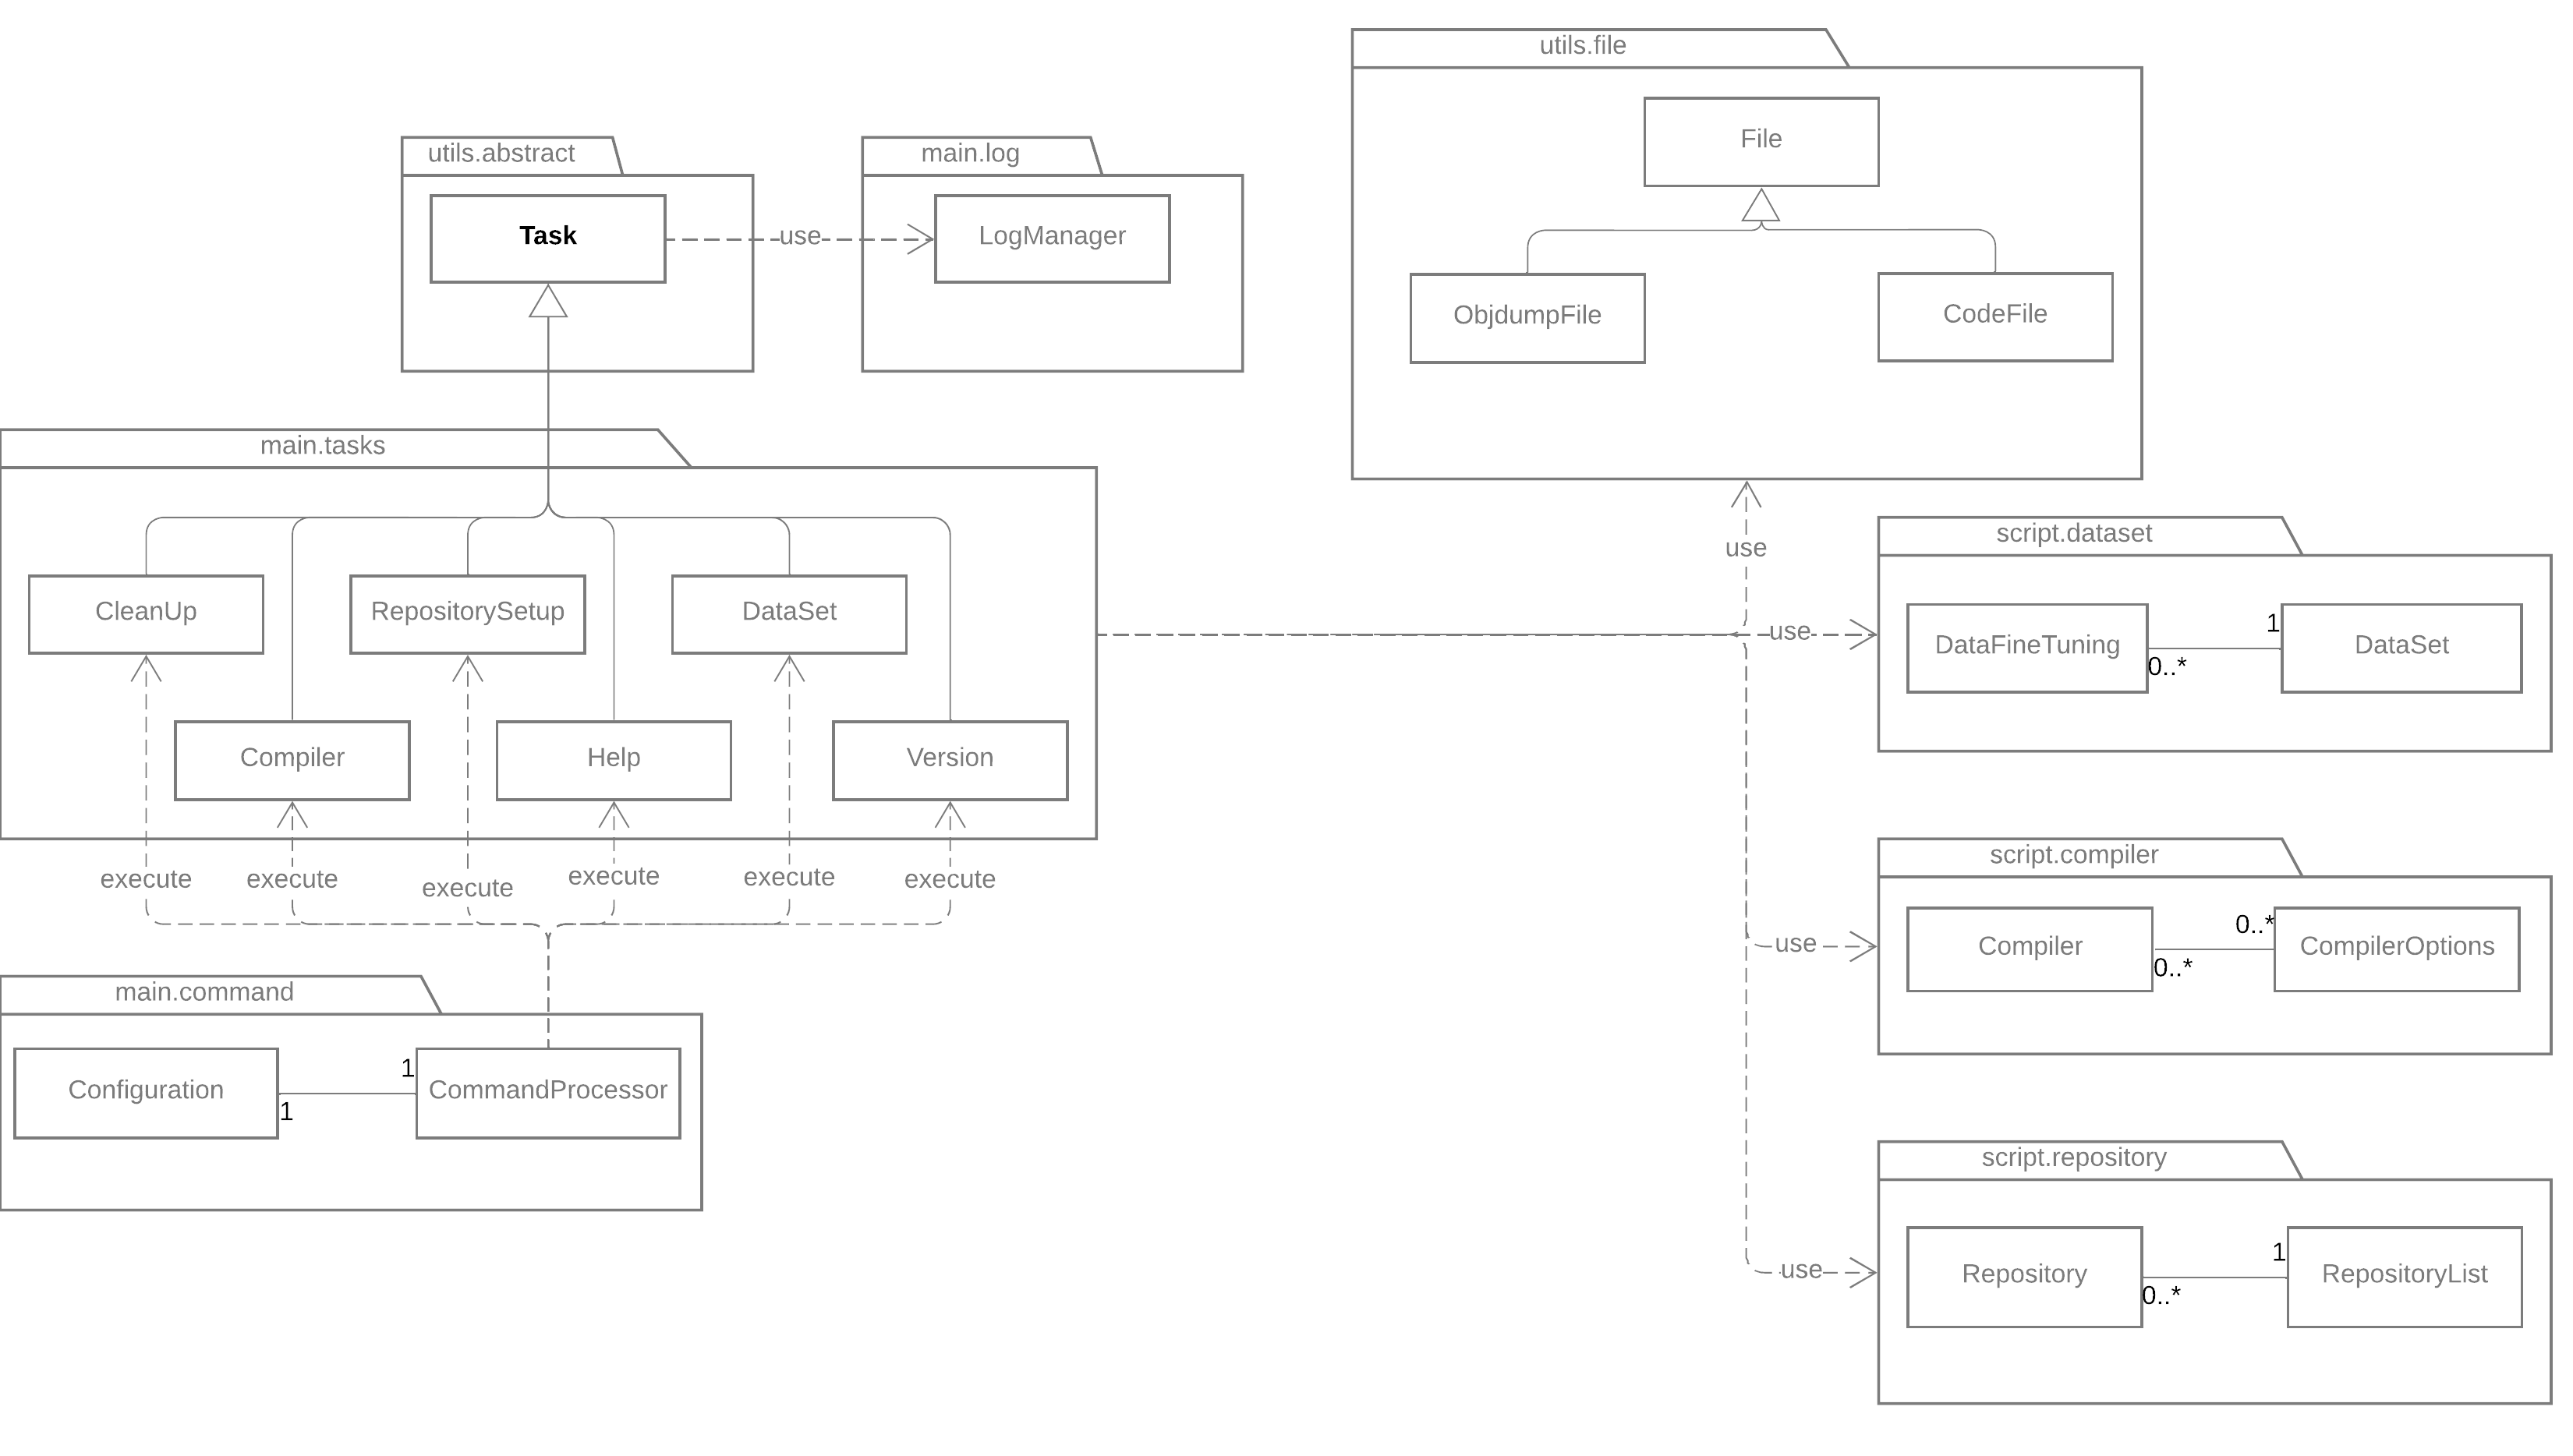
\includegraphics[scale=0.2]{figuras/Capitulo_07/UML_Script.png}
    \end{center}
    \caption[Diagrama de clases del sistema de \textit{scripts}]{Diagrama de clases del sistema de \textit{scripts} (Elaboración propia)}
    \label{fig:UML_Script}
\end{figure}\

\newpage
\paperwidth=\pdfpageheight
\paperheight=\pdfpagewidth
\pdfpageheight=\paperheight
\pdfpagewidth=\paperwidth
\headwidth=\textwidth

\section{Implementación del sistema de \textit{scripts}}
\label{sec:implementacion_sistema_scripts}

% Corregido 30/12/2023
% Revisado 14/01/2024

La implementación del sistema de \textit{scripts} se ha realizado utilizando el lenguaje de programación Python
\footnote{Python es un lenguaje de alto nivel de programación interpretado cuya filosofía hace hincapié
en la legibilidad de su código. Es un lenguaje de programación multiparadigma, ya que soporta parcialmente
la orientación a objetos, programación imperativa y programación funcional. Es un lenguaje interpretado,
dinámico y multiplataforma. }. La principal razón de utilizar este lenguaje de programación es debido a
que es un lenguaje muy orientado al \textit{scripting}, es decir, es un lenguaje que permite realizar
\textit{scripts} de manera sencilla y rápida. Además, siguiendo con los criterios de diseño que me he marcado,
Python nos permite aumentar la portabilidad de nuestro sistema, ya que es un lenguaje que se puede ejecutar
en cualquier sistema operativo.

Así mismo, Python nos permite una mayor compatibilidad con la plataforma de desarrollo elegido, que en el caso
de este proyecto es \textit{lit-gpt} que también está implementada utilizando Python. Esto nos permite
integrar nuestro sistema de \textit{scripts} con la plataforma de desarrollo de manera sencilla.

\subsection{Herramientas de desarrollo}
\label{subsec:herramientas_desarrollo}

% Corregido 30/12/2023
% Revisado 14/01/2024

Para poder desarrollar el sistema de \textit{scripts} se han utilizado diferentes herramientas de desarrollo que han 
ayudado a lo largo de la implementación del sistema. A continuación se detallan las herramientas utilizadas:

\begin{itemize}
    \item \textbf{Visual Studio Code:} es un editor de código fuente multiplataforma desarrollado por Microsoft.
        Incluye soporte para la depuración, control integrado de Git, resaltado de sintaxis, 
        finalización inteligente de código, fragmentos y refactorización de código. Es gratuito y de código abierto,
        aunque la descarga oficial está bajo software propietario y contiene características personalizadas 
        para su uso con productos y servicios de Microsoft. \cite{VisualStudioCode}
    \item \textbf{Git:} es un software de control de versiones diseñado por Linus Torvalds, pensando en la
        eficiencia y la confiabilidad del mantenimiento de versiones de aplicaciones cuando estas tienen un
        gran número de archivos de código fuente. Su propósito es llevar registro de los cambios en archivos
        y coordinar el trabajo que varias personas realizan sobre archivos compartidos. \cite{Git}
    \item \textbf{Github:} es una forja (plataforma de desarrollo colaborativo) para alojar proyectos utilizando
        el sistema de control de versiones Git. \cite{Github}
    \item \textbf{Github Copilot:} es una herramienta de programación asistida por IA que ayuda a los desarrolladores
        a escribir código. Copilot fue desarrollado por OpenAI en colaboración con GitHub. Copilot se basa en Codex,
        un modelo de lenguaje de inteligencia artificial creado por OpenAI. Copilot se anunció en junio de 2021 y
        se lanzó en versión beta en julio de 2021. \cite{GithubCopilot}
\end{itemize}

